\chapter{System Implementation And Experimental Evaluation} \label{chap:system_implementation}
    This chapter attempts to discusses the experiments performed to evaluate the proposed solutions for the implementation of the system. Section \ref{sec:development environment} provides information about the system design and choice of software and programming languages. Section \ref{sec:evaluation_of_snapshot_materialization} provides an evaluation of discussed methods for snapshot materialization by setting up different experiments. 

	\section{Development environment and application development tools} \label{sec:development environment}
		To setup the development environment of the project, we used the 'Leda' research server provided by the department of scinece at the University of Ontario Institute of Technology with the ubuntu 16.04 operating system installed. The application could be developed by various tools, but since one important goal of this project was to be able to generalize our proposed solution for majority of relational databases, we needed to choose the tools that are popular among the developers for the development of their system. For the database choice, we favored the use of postgreSQL simply because of its wide adoptation by the industry \cite{cook2017docker}. 

		The experiments scripts were mainly developed by using Python 2.7 programming language. We started off by generating a database using the TPCH schema with 1,000,000 tuples in the main table. Using Python's pycrypto 2.6.1 library \footnote{https://pypi.org/project/pycrypto/}, we developed a few functions to create digital signature of the transactions on the database system. We generated a synthetic temporal database with security information, by performing a set of random insert, delete and update transactions and by creating their digital signature at 1000 distinct timestamps. In each record, along with the digital signature of that record, we also stored the digital signature of its previous record in the temporal table. This created a Blockchain-based relational temporal table with 1,000 timestamps. 

		To be able to manage the relational database and perform queries on the tables, we utilized SQL query language. Generation of snapshots using the records stored in the temporal tables required time series analysis and performing numbers of aggregations and self-joins on the relational table. In order to make this process less cumbersome, we utilized the windowing function that is part of the SQL standard and is supported by the relational databases \cite{leis2015efficient}.

		In order to evaluate the effectiveness of snapshot materialization, the optimal snapshot placement had to be examined in different query distributions on the timeline. The Python's Numpy library gave us the ability to simulate some query distributions on the timeline. The recursion and dynamic programming experiments was performed using Python 2.7 programming language but for the heuristic method experiment, we used scikit-learn machine learning library \footnote{http://scikit-learn.org/stable/} written in Python. After running the snapshot materialization experiments and collecting data, we utilized the Python's plotly library in order to visualize the collected data.


	\section{Evaluating snapshot materialization} \label{sec:evaluation_of_snapshot_materialization}
		In this section we discuss the evaluation of snapshot materialization through different experiments. We start by showing a method to create snapshots using the temporal relation. Then we show the problem of linear computational time in performing snapshot generation on the temporal relation. Next, we evaluate the placement of a single snapshot for matrialization in different timestamps and visualize the optimal position for this purpose. In the next step we show the effectiveness of utilizing multiple number of precomputed snapshots for materialization and at the end, multiple approaches to find multiple optimal timestamps are put into different experiments.

		\subsection {Generating snapshots by using records in a temporal database} \label{sec:snapshot_generation}
			We can construct the snapshots using simple windowing functions (as is supported by PostgreSQL \cite{momjian2001postgresql}). The pseudo code of the developed function is shown in Table \ref{table:windowing_function}. 

			The query $\mathrm{snapshot}(r, t)$ computes the snapshot of $r$ at timestamp $t$ by applying the latest update of each tuple up to timestamp $t$, while removing tuples that have been deleted.
			\begin{center}
				\begin{table}[]
					\centering
					\small
						\begin{tabular}{|l|} \hline
							$\mathrm{snapshot}(r, t)$ = \\
							\verb|| \textsc{With} $T$ \textsc{as} ( \\
							\verb|   | \textsc{select} id, $\{\mathrm{last\_value}(x) \mathrm{\ as\ } x:
							x\in attr(r)\}$ \textsc{over} $W$ \\
							\verb|   | \textsc{from} $r^T$ \\
							\verb|   | \textsc{where} updates $\leq t$ \\
							\verb|   | \textsc{window} $W$ \textsc{as} 
							\textsc{partition by} id \textsc{order by} updates\\
							\verb|| ) \\
							\verb|| \textsc{select} id, $\{x: x\in attr(r)\}$ \textsc{from} $T$ \\
							\verb|| \textsc{where not} $T.$deleted \\ \hline
						\end{tabular}
				\caption{The windowing function to create snapshots}
				\label{table:windowing_function}
				\end{table}
			\end{center}

		\subsection{Evaluating the linearity of snapshot generation} \label{sec:evaluating_linearity}
			To prove the linearity of snapshot generation experimentally, we developed an experiment to create and record runtime of 100 snapshots on the timeline of temporal database. Using the resulted runtime data, the cost-line was visualized which is shown if Figure \ref{fig:linear_time}. Note that the runtime is in seconds.

			Figure \ref{fig:linear_time} clearly proves our claim that computation of snapshots on a temporal table requires linear time. The issue of linearity in computation of snapshots makes such tasks on a very large table inefficient.

			\begin{figure}[]
				\centering
				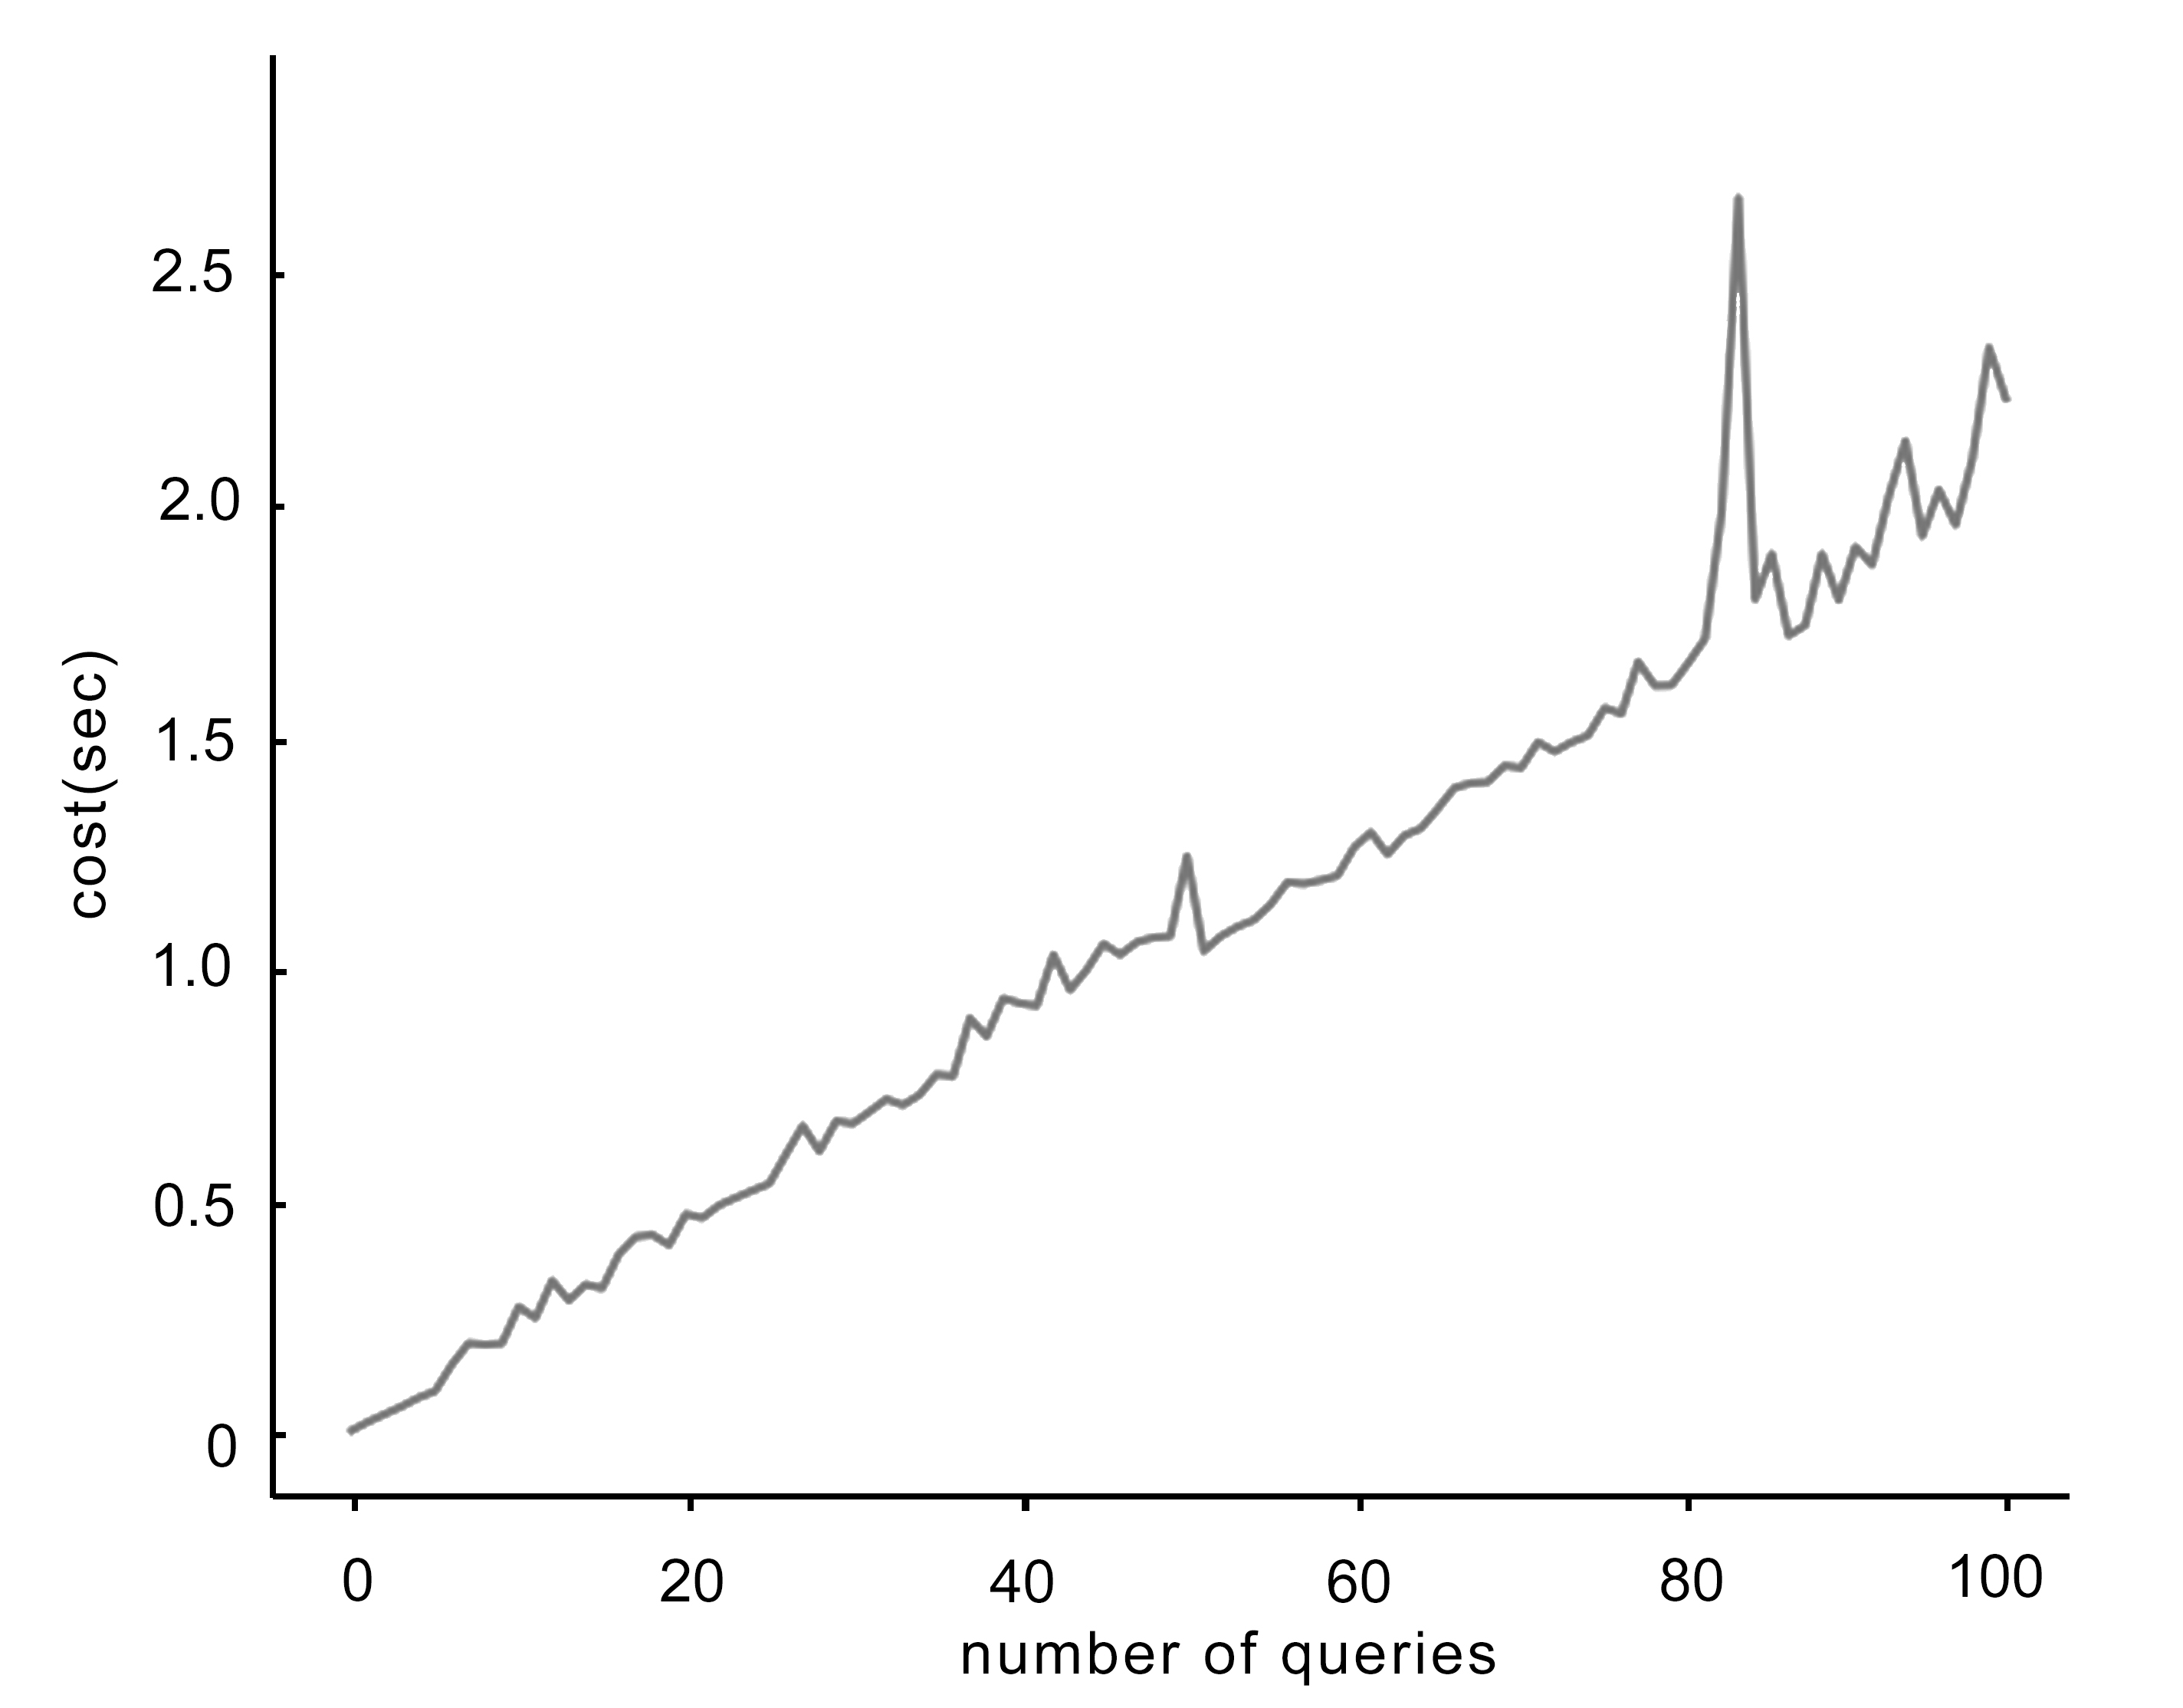
\includegraphics[width=120mm]{figs/runtime.jpg}
				\caption{Linear time in computation of snapshots without snapshot materialization}
				\label{fig:linear_time}
			\end{figure} 
		\subsection{Evaluating materialization of a single snapshot} \label{sec:evaluating_single_snapshot}
			The purpose of this experiment is to visually see that the optimal timestamp of a single snapshot for materialization is the median of previousely performed queries. For this purpose we randomly sampled 60 query timestamps from our temporal database timeline. Each query was genrating an snapshot of the relation at an specific timestamp. In the next step we placed a single snapshot for these queries to materialize and computed the overal cost of query answering using definition \ref{defn:cost_of_query_answering}. To see the effects of repositioning the materialized snapshot on the timeline, we slided the materialized snapshot on the timeline of the temporal relation. The resulted overall cost-line obtained from sliding the snapshot is depicted in Figure \ref{fig:single_snapshot}. 

			The resulted cost line shown in Figure \ref{fig:single_snapshot} clearly shows that the position of a snapshot directly affects the overal cost of query answering on the temporal table. We also computed the median of the queries on the timeline which is seen as a red dot on the figure. As seen in the figure, the median of the queries is indeed located in the position where the cost-line's global minimum is. This proves that the median of the queries is the most optimal position to place a single snapshot for materialization.

			\begin{figure}
				\centering
				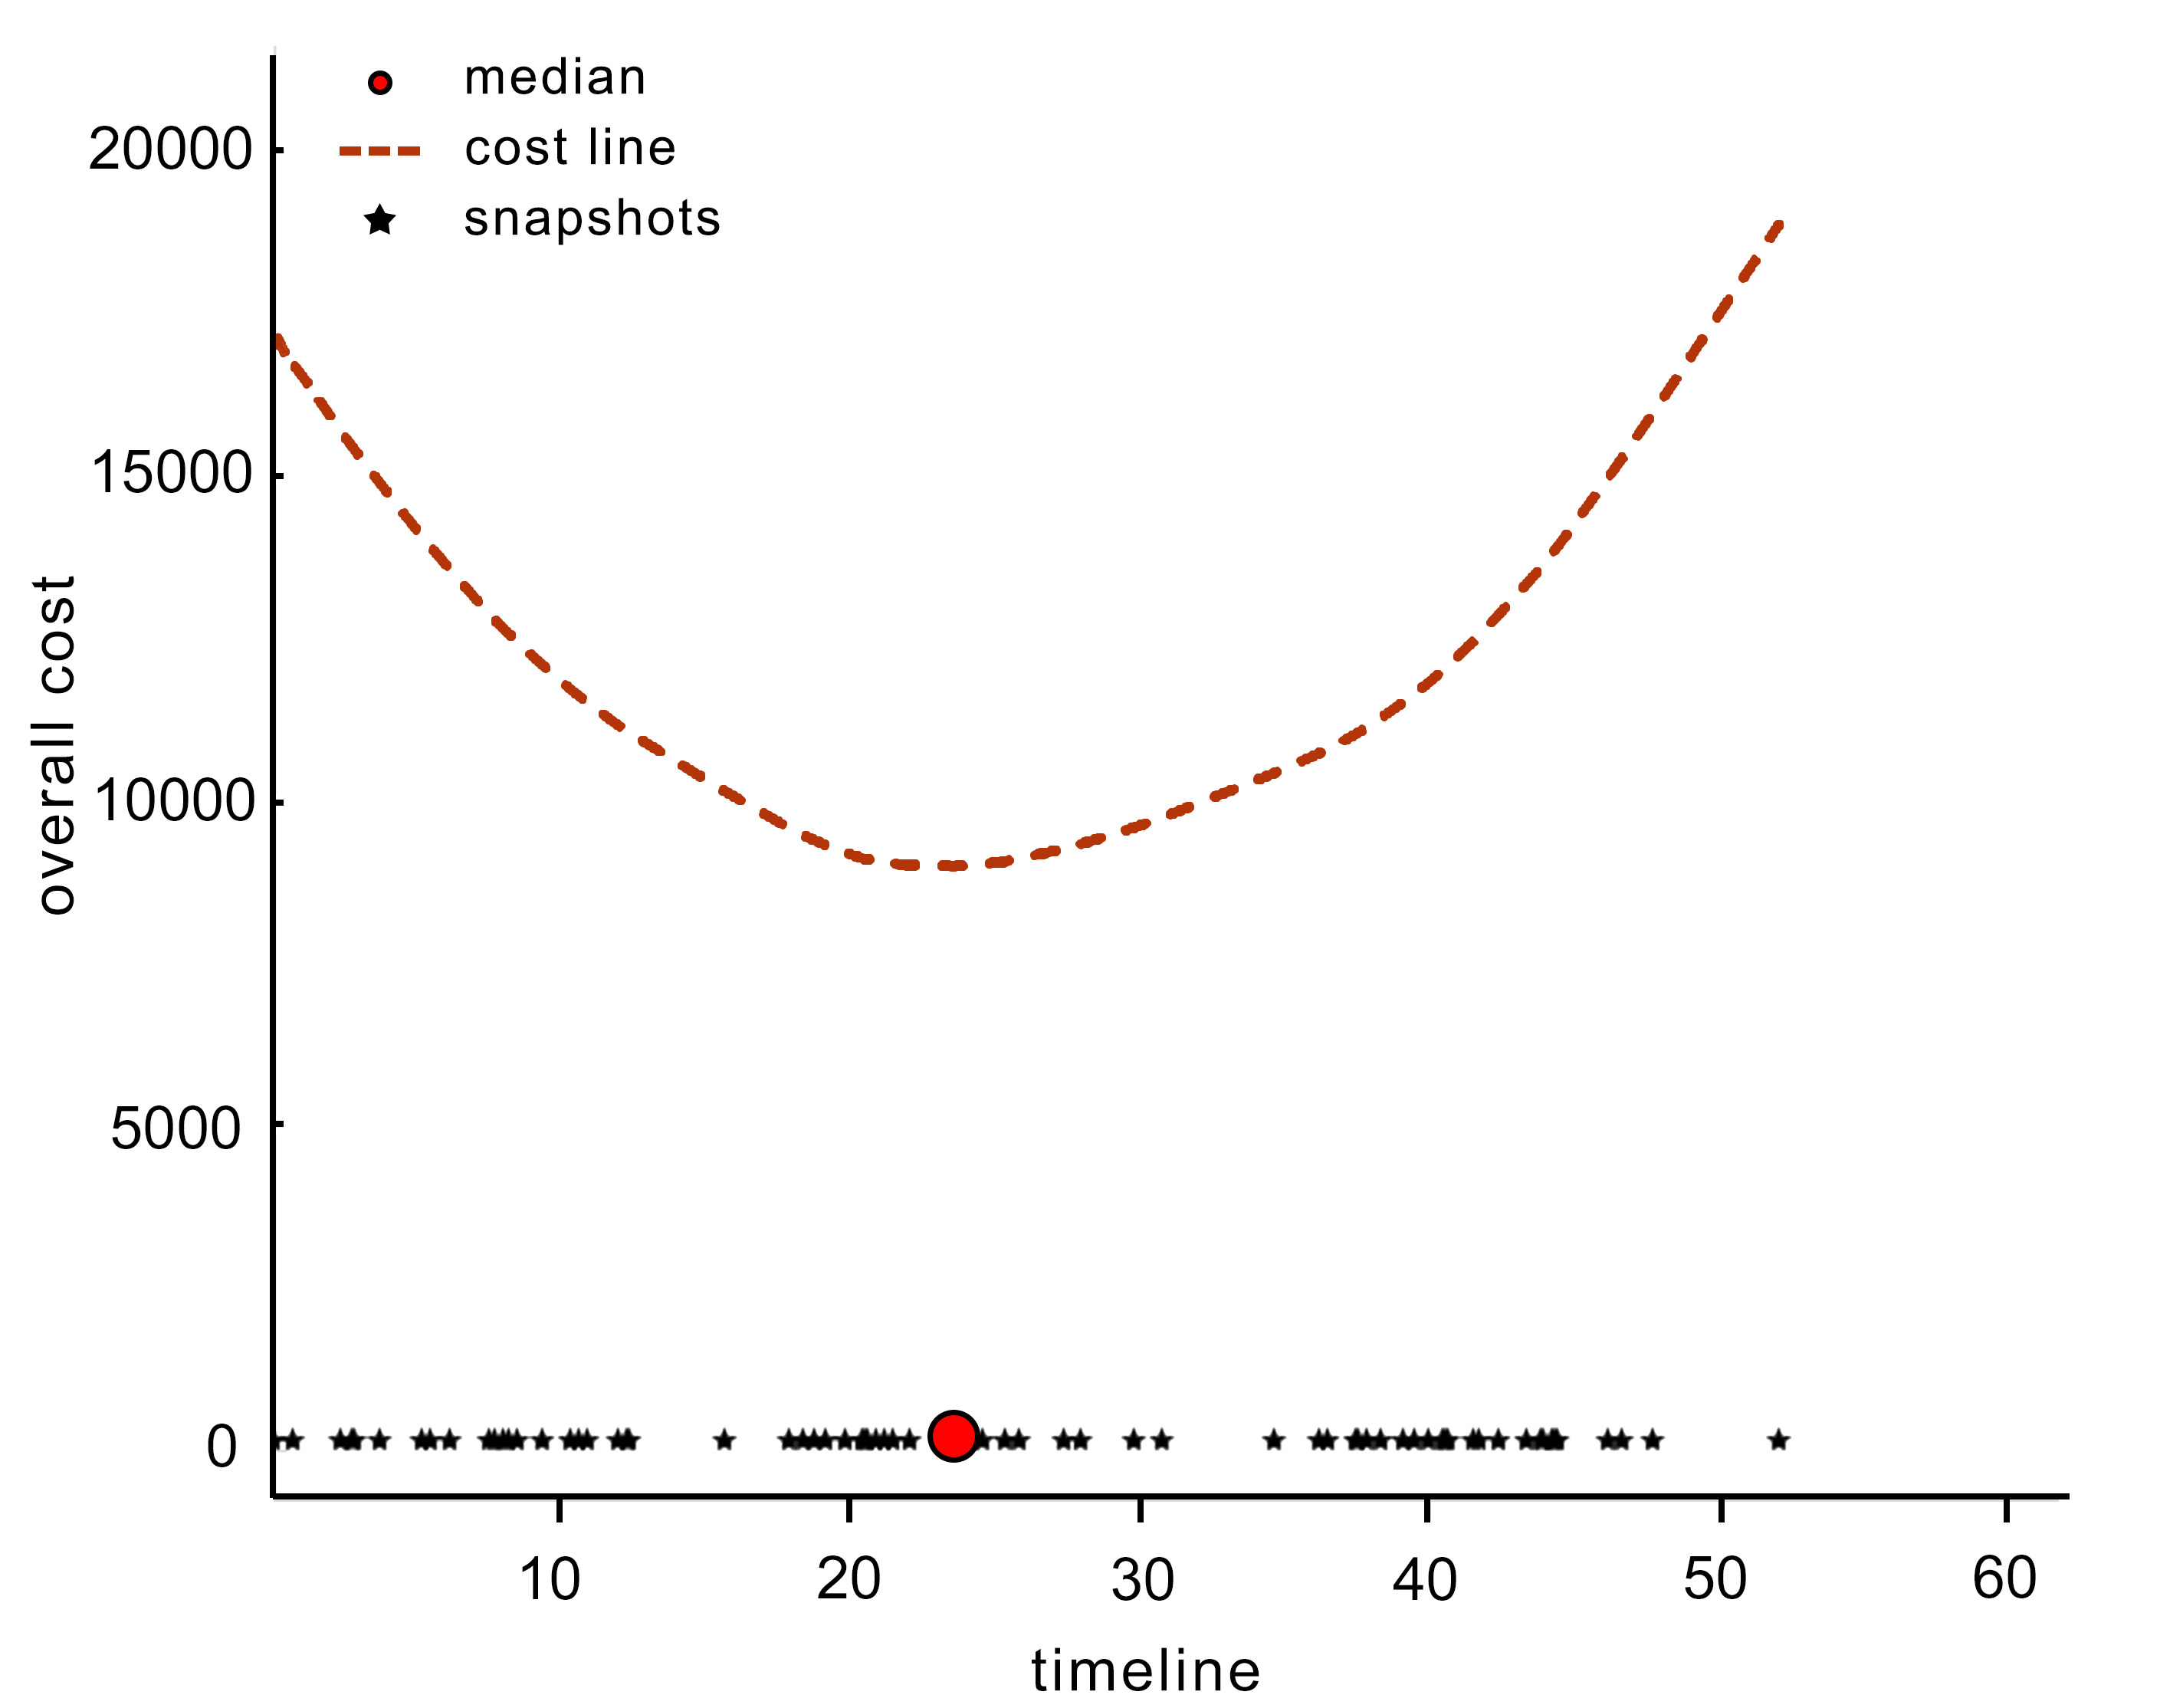
\includegraphics[width=90mm]{figs/single_snapshot.jpg}
				\caption{Cost of query answering using a single snapshot over different snaptshot timestamps}
				\label{fig:single_snapshot}
			\end{figure} 

		\subsection{Evaluating materialization of multiple snapshot} \label{evaluating_multiple_snapshots}
			To evaluate the performance of our optimal snapshot computation, we evaluated the recursive formulation given
			by Section \ref{sec:optimal_recursive_segmentation}, the dynamic programming formulation given by Section \ref{sec:dynamic_programming_optimal_segment} and heuristic method given by Section \ref{sec:heuristic_optimal}. 

			To illustrate that the optimal snapshot placement indeed produces the best query answering performance, we compared the query answering cost of three approaches:
			\begin{itemize}
				\item Pick $m$ random timestamps to place the snapshots.
				\item Pick $m$ evenly intervaled timestamps to place the snapshots.
				\item Pick $m$ timestamps computed by dynamic programming.
			\end{itemize}

			\begin{figure}
				\centering
				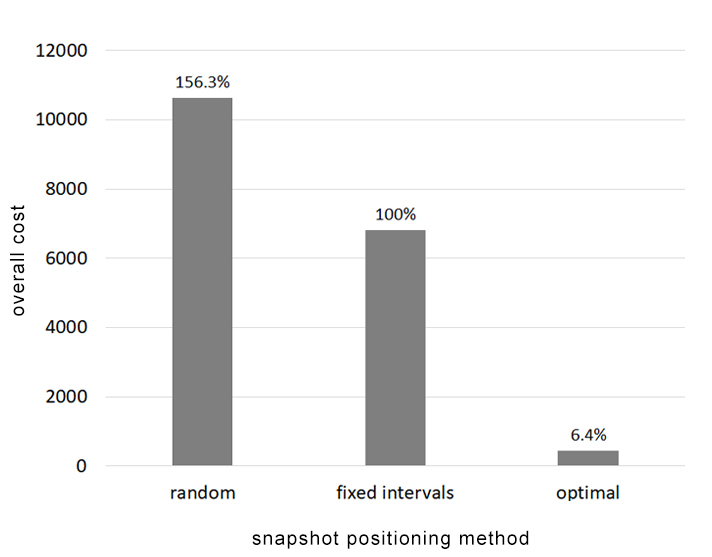
\includegraphics[width=80mm]{figs/various_scenarios_cost.jpg}
				\caption{Query answering cost with forty snapshots with various approaches to place snapshots for materialization}
				\label{fig:approaches_cost}
			\end{figure} 

			Figure \ref{fig:approaches_cost} shows that the placements obtained by dynamic programming clearly beats the other two approaches.

			In order to evaluate the effectiveness of $m$ number of snapshots to lower the overal cost of query answering, we recorded the overal cost of queries in various number of snapshots. Figure \ref{fig:snapshots_cost} shows that as the number of snapshots for materialization increases, the overal cost of answering to the queries drops.

			\begin{figure}
				\centering
				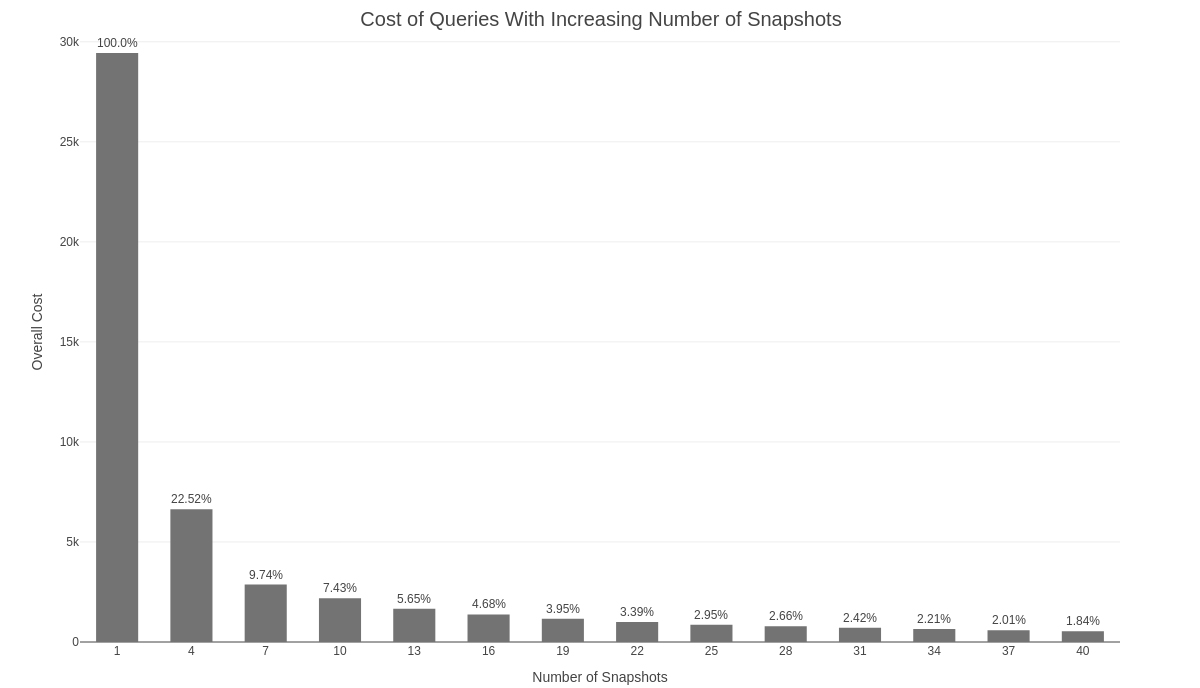
\includegraphics[width=\textwidth]{figs/various_snapshot.jpg}
				\caption{Query answering cost with increasing number of snapshots}
				\label{fig:snapshots_cost}
			\end{figure} 

		\subsection{Implementation of recursive algorithm} \label{sec:recursive_implementation}
			Recursive method was our first approach to find $m$ number of optimal segmentations of the timeline for snapshot placement. The recursive algorithm of this operation is given as Algorithm \ref{alg:recursive}.

			\begin{algorithm}
				\SetAlgoLined
				\caption{Recursive algorithm method to compute $m$ number of optimal segmentations}
				\SetAlCapNameFnt{\tiny}
				\label{alg:recursive}
				\DontPrintSemicolon
				 \SetKwFunction{FMain}{computeOPT}
				 \SetKwProg{Fn}{Function}{:}{}
				 \Fn{\FMain{$Q$, $m$}}{
				    $n = |Q|$\;
				    \textbf{OPT}$[i,0]$ = $\infty$ \;
				    \For{$k \gets 1$ \KwTo $m$}{
				    	\For{$i \gets 1$ \KwTo $n$}{
				    		$j^* = \underset{j\in[1,i]}{\mathrm{argmin}}(\mathrm{cost}(\mathbf{OPT}[j,k-1]) + \mathrm{cost}(Q[j+1, n]))$ \;
				    		$\mathbf{OPT}[i,k] = \mathbf{OPT}[j^*, k-1] \cup \{\mathrm{median}(Q[j+1], n)\}$ 
				    	}
				    }
				}
			\end{algorithm}

		\subsection{Implementation of dynamic programming} \label{sec:dynamic_implementation}
			Dynamic programming was the second approach that we utilized in order to find $m$ number of optimal segmentation of the timeline for snapshot placement. The dynamic programming uses the memoization technique in which the algorithm stores the result of an expensive function calls in a table, and retrieve the result from the table, when the same inputs to the function is given. This approach could be implemented using Algorithm \ref{alg:dynamic_programming}.
			\begin{algorithm}
				\SetAlgoLined
				\caption{Dynamic programming method to compute $m$ number of optimal segmentations}
				\SetAlCapNameFnt{\tiny}
				\label{alg:dynamic_programming}
				\DontPrintSemicolon
				 \SetKwFunction{FMain}{computeOPT}
				 \SetKwProg{Fn}{Function}{:}{}
				 \Fn{\FMain{$Q$, $m$}}{
				    $n = |Q|$\;
				    $minVal = \infty$ \;
				    \For{$i \gets 1$ \KwTo $m$}{
				    	\For{$j \gets 1$ \KwTo $n+1$}{
				    		\For{$k \gets 1$ \KwTo $j$}{
				    			$minVal = \mathrm{min}(\textrm{minVal},\mathbf{Table}[i,k] + \mathrm{cost}(Q[j-k:]))$
				    		}
				    	$\mathbf{Table}[i,j] = minVal$
				    	}
				    }
				}
			\end{algorithm}


		\subsection{Implementation of heuristic method} \label{sec:implementation_heuristic}
			To evaluate the performance of heuristic method in finding $m$ number of optimal segmentation of the timeline for snapshot placement, we chose K-means clustering method. Although the K-means clustering method doesnot guarantee the most optimal solution of creating the segmentations, but we expect a satisfactory results obtained from this method.

			The K-means clustering algorithm is given as Algorithm \ref{alg:Kmeans}.
			\begin{algorithm}
				\SetAlgoLined
				\caption{K-means clustering to compute $m$ number of segmentations}
				\label{alg:Kmeans}
				\DontPrintSemicolon
				 \SetKwFunction{FMain}{K-Means}
				 \SetKwProg{Fn}{Function}{:}{}
				 \Fn{\FMain{$T_q^*\{q_1,...,q_n\}$, $m$, maxIteration}}{
				 $iteration \gets 0$ \;
				 \Repeat{$convergence$ and $iteration \leq maxIteration$}{
				    $\{\mu_1,...,\mu_m\} \gets SelectRandomSeeds(\{q_i\in T_q^*\},m)$ \;
					\For{$i \gets 1$ \KwTo $n$}{
						$J \gets argmin_{J^*}||\mu_{J^*}-q_i||^2$ \;
						$\mathcal{L}_j \gets \mathcal{L}_j \cup \{q_i\}$ 
					}
					\For{$j \gets 1$ \KwTo $m$}{
						$\mu_j \gets \frac{1}{\mathcal{L}_j} \sum_{q \in \mathcal{L}_j} q $
					}
					$iteration ++$
				}
					\Return\{$\mu_1,...,\mu_m$\}
				}
			\end{algorithm}

		\subsection{Evaluating approaches for optimal placement of $m$ snapshots} \label{sec:evaluating_approaches}
			 In this research, we examine three approaches to find the optimal timestamps for $m$ number of snashots for materialization. The performed approaches are:
			\begin{itemize}
				\item Recursive algorithm.
				\item Dynamic programming.
				\item K-Means clustering.
			\end{itemize}
			\subsubsection {Experiment 1.} \label{sec:experiment_1}
			In the first experiment , we evaluate the performance of each approach with respect to fixed number of queries and variable number of snapshots For this experiment we sampled 140 number of queries and evalueted the runtime of each approach while increasing the number of requested snapshots.

			\begin{figure}
				\centering
				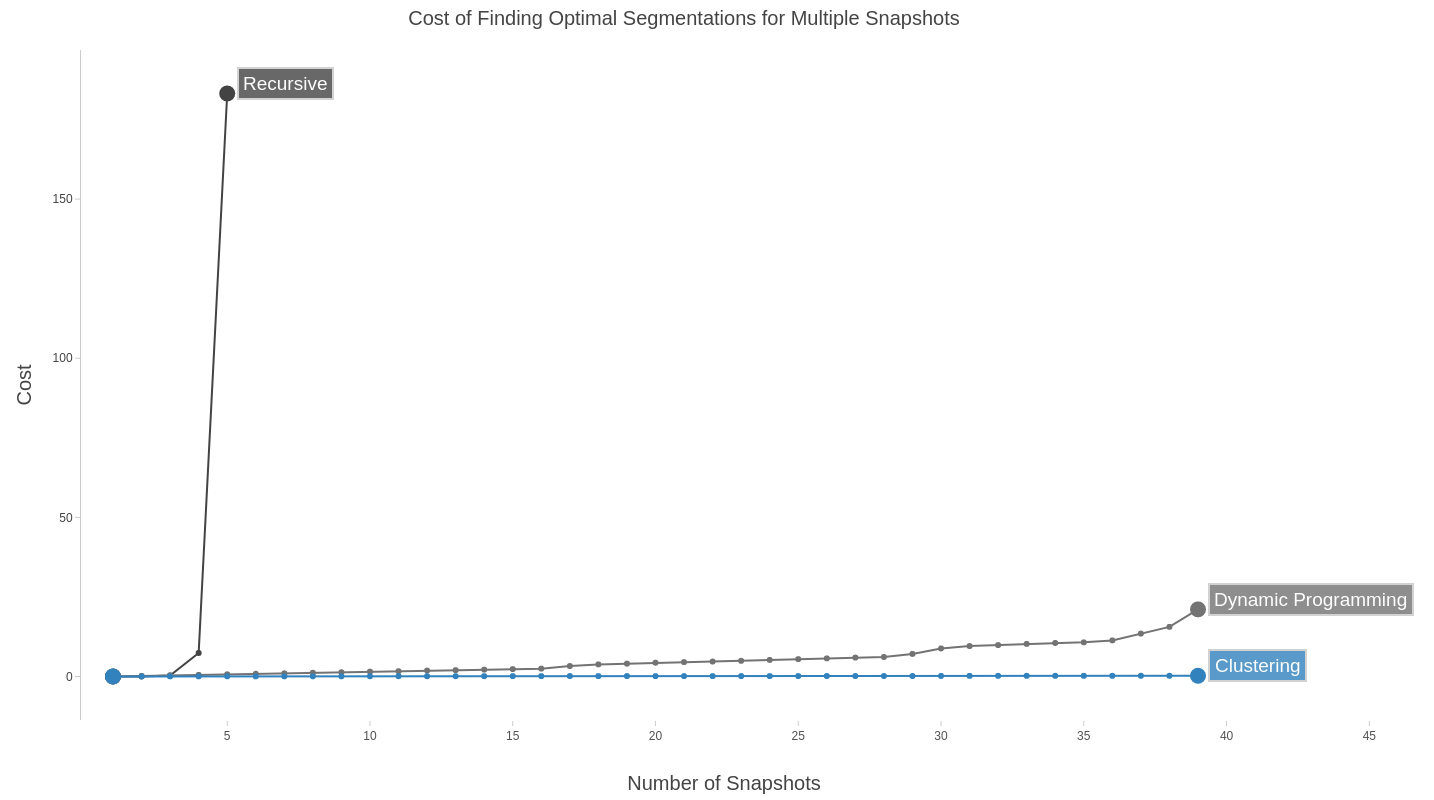
\includegraphics[width=\textwidth]{figs/variable_snapshots.jpg}
				\caption{Optimization runtime with respect to the number of snapshots (in seconds)}
				\label{fig:variable_snapshots}
			\end{figure} 

			\begin {center}
			\begin{table}
				\centering
				\caption{Optimization runtime with respect to the number of snapshots}
				\label {table:variable_snapshots}
				\begin{tabular}{p{2cm}p{3cm}p{3cm}p{3cm}}
					\hline
					Snapshots & Recursive (sec)     & Dynamic (sec) & Clustering (sec) \\ \hline
					1 & 0.0002    & 0.01  & 0.01  \\  
					2 & 0.01    & 0.17  & 0.02  \\
					3 & 0.32    & 0.34  & 0.03  \\
					4 & 7.39 & 0.52  & 0.04  \\
					5 & 183.18 & 0.69  & 0.06 \\
					10 & N/A    & 1.52  & 0.08  \\
					15 & N/A & 2.33  & 0.12  \\ 
					20 & N/A & 4.33  & 0.12  \\ 
					25 & N/A & 5.46  & 0.14  \\ 
					30 & N/A & 8.81  & 0.17  \\
					35 & N/A & 10.74  & 0.21  \\
					40 & N/A & 21.09  & 0.24  \\\hline
				\end{tabular}
			\end{table}
			\end{center}

			Figure \ref{fig:variable_snapshots} and Table \ref{table:variable_snapshots} depict the observations of the experiment. The graph shows that in comparison with dynamic programming and K-means clustering, the recursive algorithm is computationally more expensive. In fact we could not find the optimal timestamp for more than five snapshots because the results did not converge.

			\begin{figure}
				\centering
				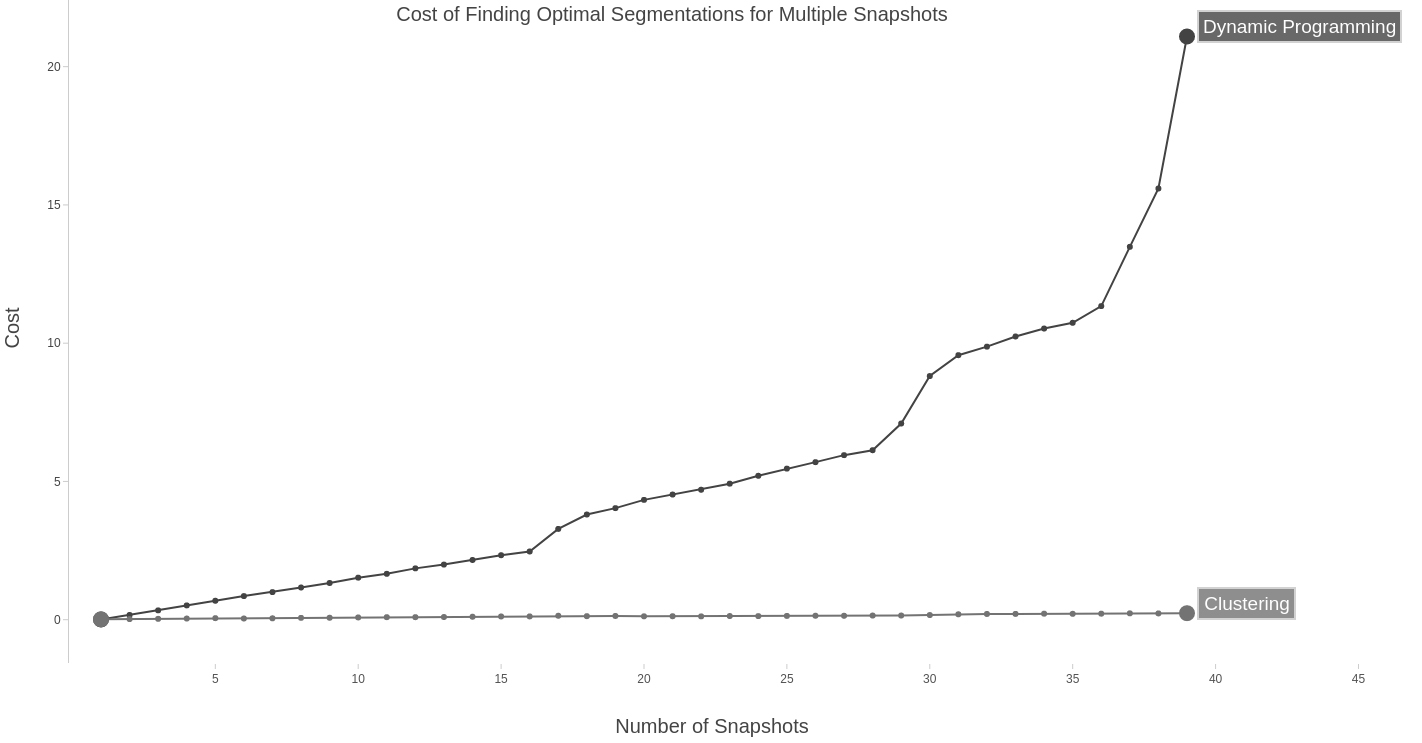
\includegraphics[width=\textwidth]{figs/multiSnapDouble.jpg}
				\caption{Optimization runtime with respect to the number of snapshots (in seconds)}
				\label{fig:variable_snapshots_2}
			\end{figure} 

			\begin{center}
			\begin{table}
				\centering
				\caption{Optimization runtime with respect to the number of snapshots}
				\label {table:variable_snapshots_2}
				\begin{tabular}{p{2cm}p{3cm}p{3cm}}
					\hline
					Snapshots  & Dynamic (sec) & Clustering (sec)\\ \hline
					1 &   0.01 & 0.01 \\  
					2 &  0.17  & 0.02  \\
					3 &  0.34  & 0.03  \\
					4 & 0.52  & 0.04  \\
					5 &  0.69  & 0.06 \\
					10 &  1.52  & 0.08  \\
					15 & 2.33  & 0.12  \\ 
					20 & 4.33  & 0.12  \\ 
					25 & 5.46  & 0.14  \\ 
					30 & 8.81  & 0.17  \\
					35 & 10.74  & 0.21  \\
					40 & 21.09  & 0.24  \\\hline
				\end{tabular}
			\end{table}
			\end{center}
			Figure \ref{fig:variable_snapshots} and Table \ref{table:variable_snapshots_2}, have a closer look at the dynamic programming and clustering method. As it could be seen, the clustering technique finds the optimal timestamps for the snapshots in a lower runtime.

			\subsubsection {Exmperiment 2.} \label{sec:experiment_2}

			In the second experiment of this category, we evaluated the three approaches of finding optimal timestamps for fixed the number of snapshots and variable number of queries. For this reason, we computed 4 number of optimal timestamps for queries ranging from 12 to approximately 180. 

			\begin{figure}
				\centering
				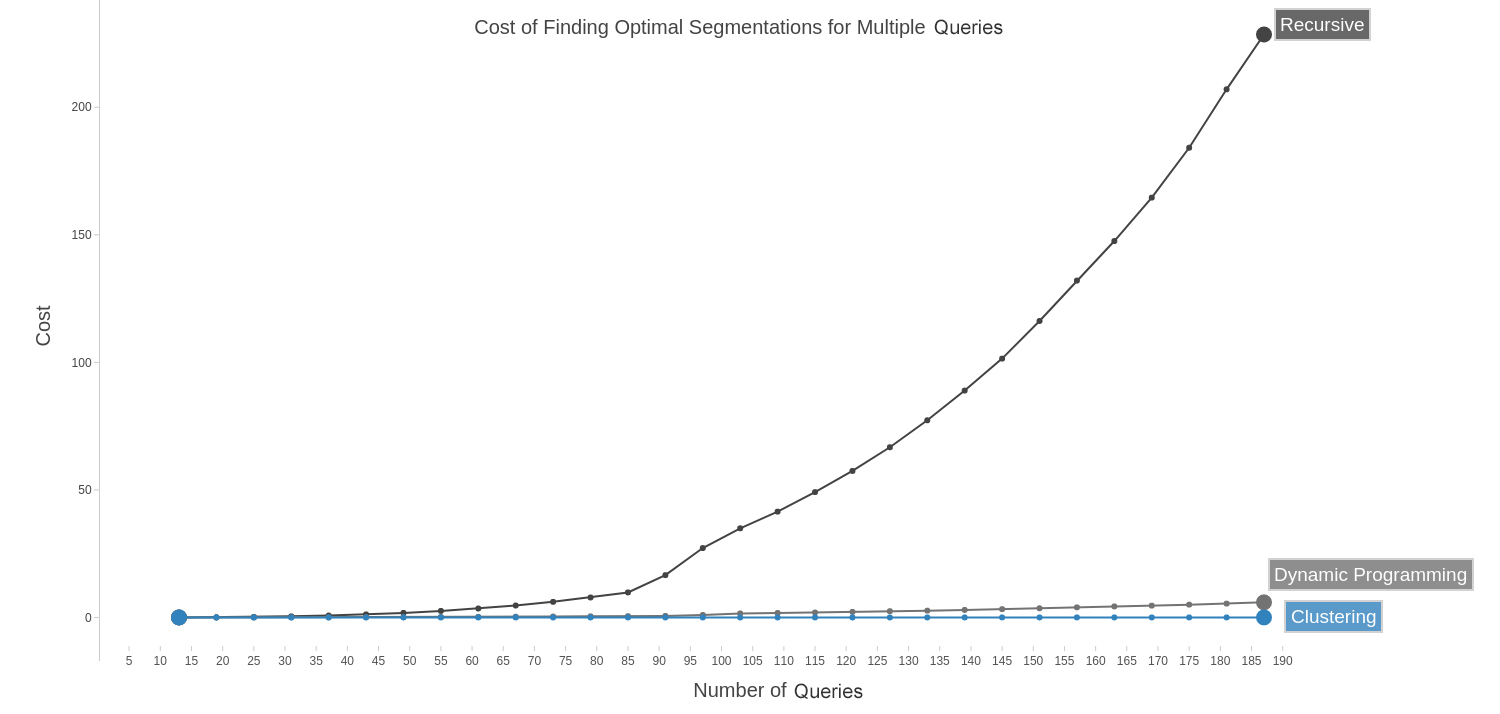
\includegraphics[width=\textwidth]{figs/multi_query.jpg}
				\caption{Optimization runtime with respect to the number of queries (in seconds)}
				\label{fig:variable_queries}
			\end{figure} 


			\begin {center}
			\begin{table}
				\centering
				\caption{Optimization runtime with respect to the number of queries}
				\label {table:variable_queries}
				\begin{tabular}{p{2cm}p{3cm}p{3cm}p{3cm}}
					\hline
					Queries & Recursive (sec)   & Dynamic (sec)  & Clustering (sec) \\ \hline
					13 & 0.05   & 0.01  & 0.02  \\  
					43 & 1.23   & 0.13  & 0.03  \\
					73 & 6.15   & 0.39  & 0.03  \\
					103 & 34.98 & 1.60  & 0.03  \\
					133 & 77.31 & 0.69  & 0.04 \\
					163 & 147.57 & 4.35  & 0.04  \\
					187 & 228.52 & 5.96  & 0.04  \\\hline
				\end{tabular}
			\end{table}
			\end{center}

			Figure \ref{fig:variable_queries_2} and Table \ref{table:variable_queries_2} shows that similar to the previous experiment, recursive algorithm has proven to be expensive in computing the optimal timestamps of the snapshots. Figure \ref{fig:variable_queries_2} and Table \ref{table:variable_queries_2} also compares the dynamic programming with heuristic method.

			\begin{figure}
				\centering
				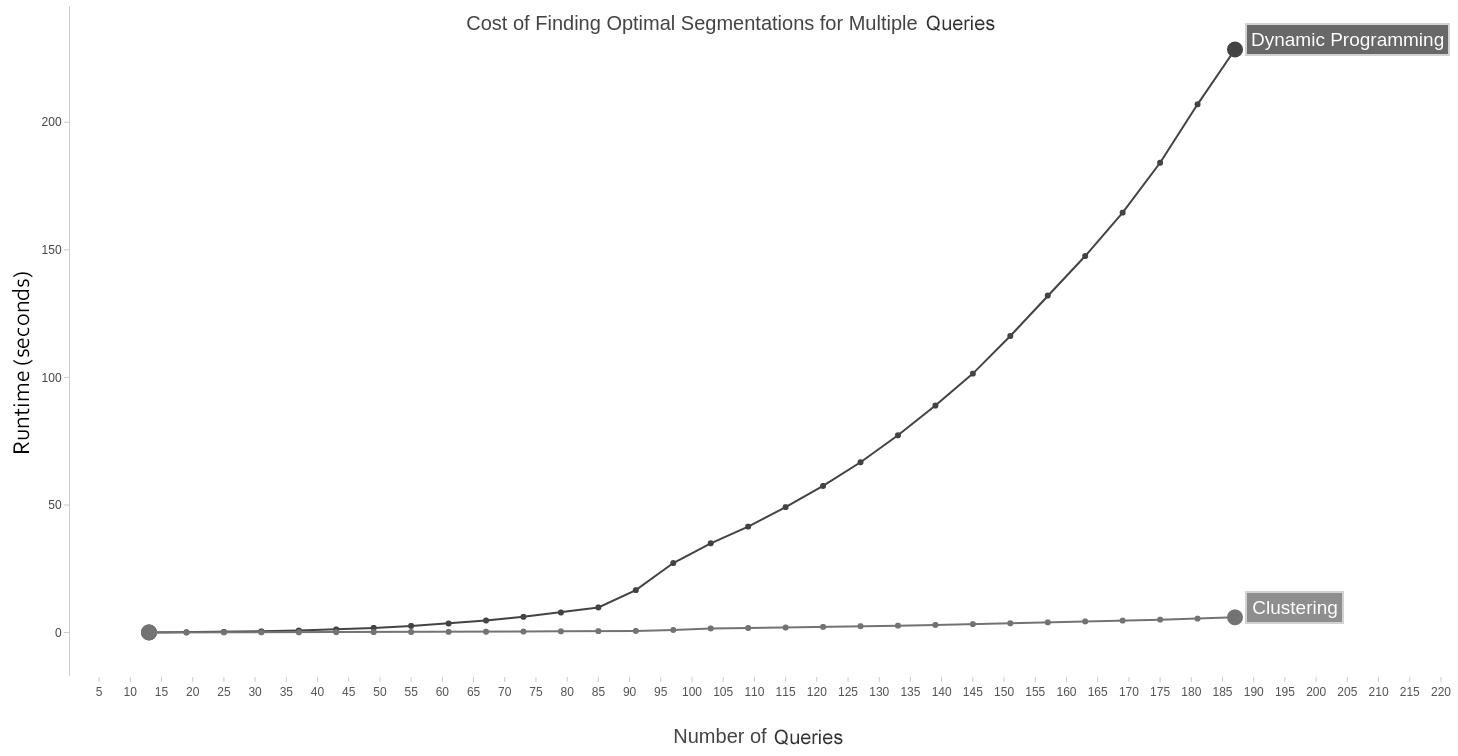
\includegraphics[width=\textwidth, scale=0.5]{figs/multi_query_2.jpg}
				\caption{Optimization runtime with respect to the number of queries (in seconds)}
				\label{fig:variable_queries_2}
			\end{figure} 


			\begin {center}
			\begin{table}
				\centering
				\caption{Optimization runtime with respect to the number of queries (in seconds)}
				\label {table:variable_queries_2}
				\begin{tabular}{p{2cm}p{3cm}p{3cm}p{3cm}}
					\hline
					Queries  & Dynamic (sec) & Clustering (sec) \\ \hline
					13 & 0.01  & 0.02  \\  
					43 & 0.13  & 0.03  \\
					73 & 0.39  & 0.03  \\
					103 & 1.60  & 0.03  \\
					133 & 0.69  & 0.04 \\
					163 & 4.35  & 0.04  \\
					187 & 5.96  & 0.04  \\\hline
				\end{tabular}
			\end{table}
			\end{center}

			The results obtained from these set of experiments show that, the heuristic method is computationally more favorable than the other two methods. When in a system, the {\it{exact optimal}} solution has more priority over the runtime, the dynamic programming could be seen as a better option. However in largescale systems that the runtime is more important, heuristic method could be more favorable. Mobile systems are one example in which the runtime matters the most. 

			\subsection{Evaluating the heuristic method} \label{sec:evaluating_heuristic}
			Since heuristic method does not guarantee the {\it exact} optimal solution, we tend to compare the solution obtained from heuristic method with the {\it exact} optimal solution obtained from dynamic programming method. Our objective was to see if the heuristic method returns satisfactory results. 
			In this experiment, we compared the outcome of the dynamic programming and K-Means clustering method in varying number of snapshots but fixed number of queries (160 queries). Figure \ref{fig:dynamic_vs_heuristic} and Table \ref{table:dynamic_vs_heuristic} show that the 
			difference from outcome of dynamic programming and heuristic method is slight, and the heuristic method has a satisfactory results.

			\begin{figure}
				\centering
				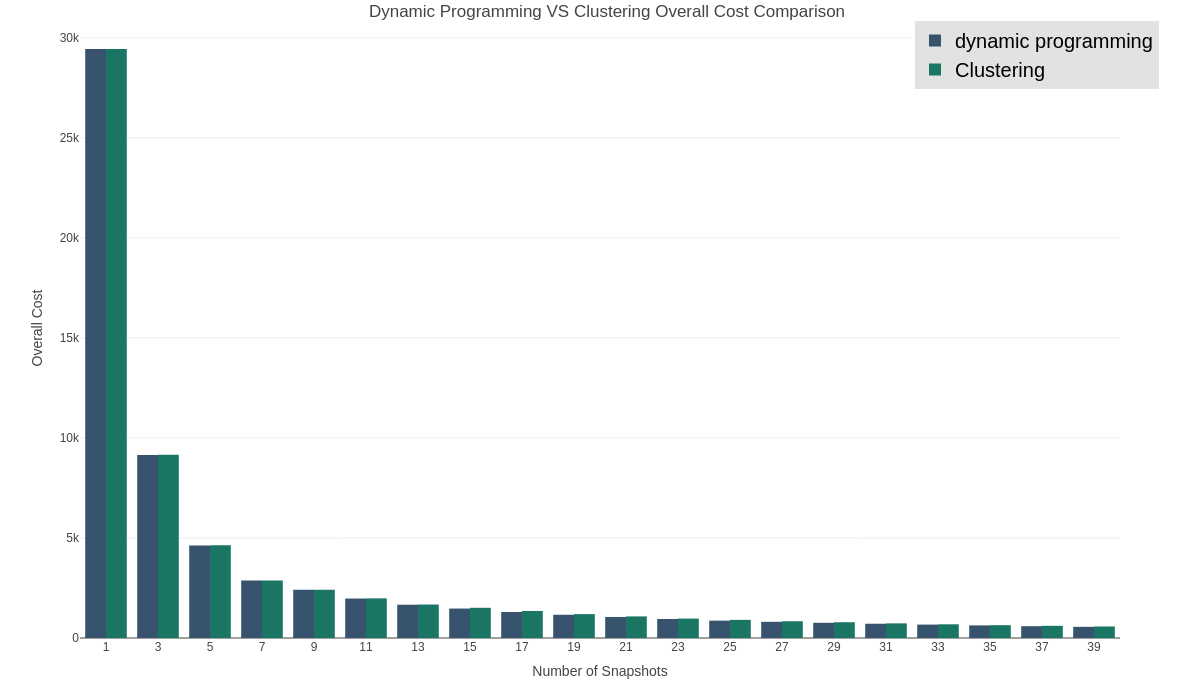
\includegraphics[width=\textwidth]{figs/dynamic_vs_clustering.jpg}
				\caption{Comparing the outcome of dynamic programming with the heuristic method}
				\label{fig:dynamic_vs_heuristic}
			\end{figure} 

			\begin {center}
			\begin{table}
				\centering
				\caption{Comparing the outcome of dynamic programming with the heuristic method}
				\label {table:dynamic_vs_heuristic}
				\begin{tabular}{p{2cm}p{3cm}p{3cm}p{3cm}}
					\hline
					Snapshots & Dynamic & Clustering \\ \hline
					1 & 29439.26  & 29439.26  \\  
					3 & 9141.55  & 9159.13  \\
					5 & 4626.77  & 4630.08  \\
					7 & 2867.74  & 2867.74  \\
					9 & 2410.46  & 2412.62 \\
					11 & 1972.14  & 1980.95  \\
					13 & 1664.14  & 1673.32  \\
					15 & 1471.58  & 1509.57  \\
					17 & 1300.32  & 1351.44  \\
					19 & 1162.25  & 1194.61  \\
					21 & 1051.97  & 1079.71  \\
					23 & 951.06  & 970.72  \\
					25 & 867.35  & 907.30  \\
					27 & 810.01  & 836.97  \\
					29 & 759.69  & 787.86  \\
					31 & 713.04  & 731.61  \\
					33 & 670.39  & 684.13  \\
					35 & 629.69  & 640.58  \\
					37 & 591.08  & 608.96  \\
					39 & 557.81  & 575.97  \\\hline
				\end{tabular}
			\end{table}
			\end{center}

			The K-means clustering method used in the experiments used 300 itterations until the solution is converged. For the purpose of lowering the runtime even more, we lowered the number of iterations to 30 and performed the experiments again. Figure \ref{fig:clustering_comparison_multiQuery} shows the runtime comparison of K-Means clustering method with 300 iterations and 30 iterations for fixed number of queries but variable number of snapshots and Figure \ref{fig:clustering_comparison_multiSnap} shows the same comparison for fixed number of snapshots but varying number of queries.

			\begin{figure}
				\centering
				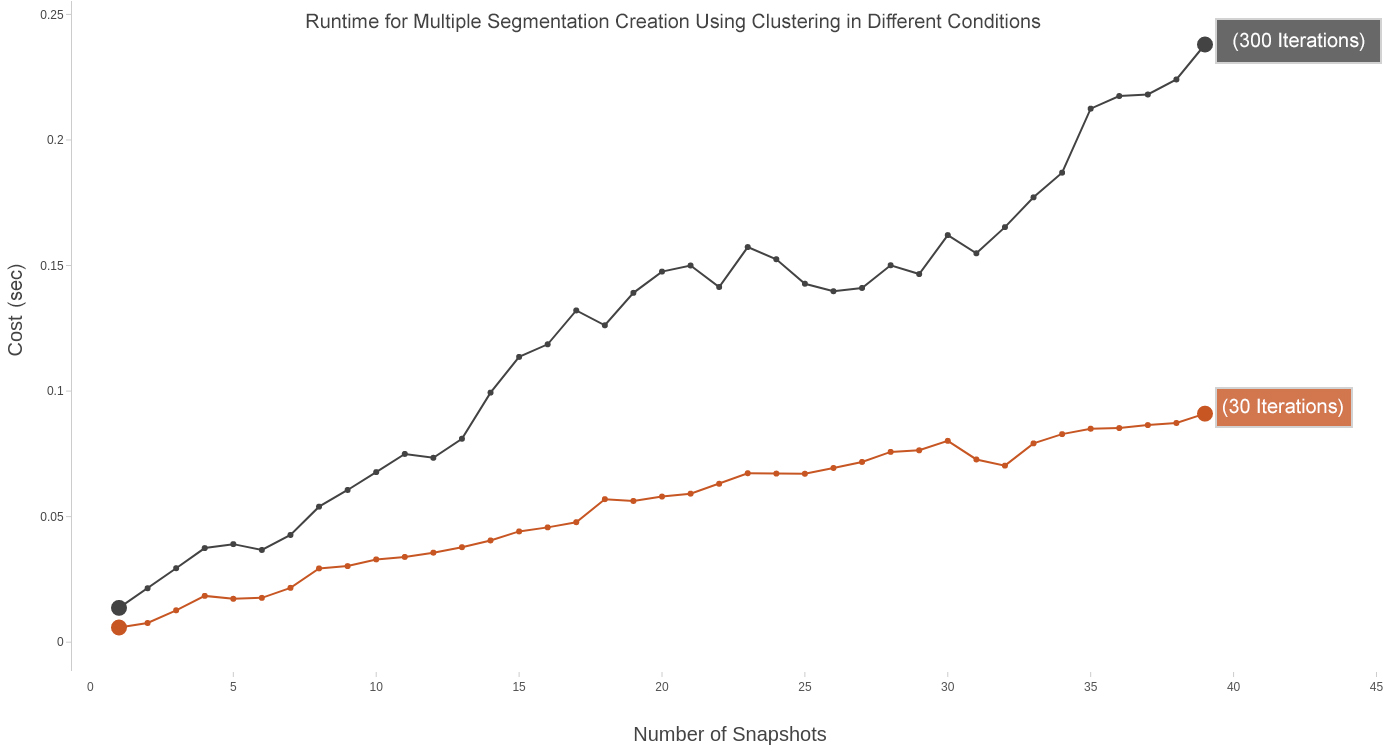
\includegraphics[width=\textwidth]{figs/multiSnap_clustering.jpg}
				\caption{Comparing the runtime of K-Means clustering method with 30 and 300 iterations for variable number of snapshots}
				\label{fig:clustering_comparison_multiSnap}
			\end{figure} 

			\begin{figure}
				\centering
				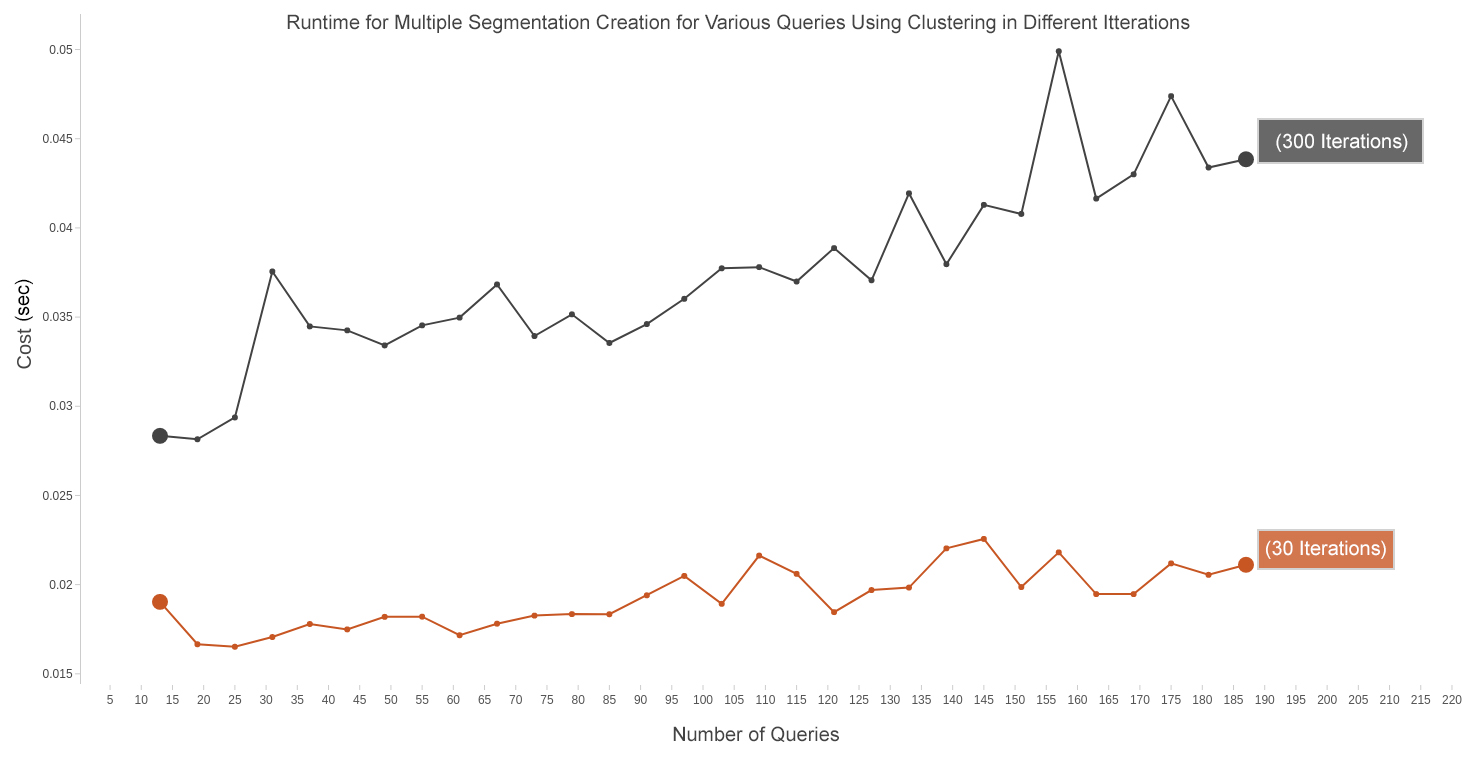
\includegraphics[width=\textwidth]{figs/multiQuery_clustering.jpg}
				\caption{Comparing the runtime of K-Means clustering method with 30 and 300 iterations for variable number of queries}
				\label{fig:clustering_comparison_multiQuery}
			\end{figure} 

			Then we compared the overal cost of query answering with the same setting in variable number of snapshots. As it could be inferred from Figure \ref{fig:compare_clusterings_iterations} and Table \ref{table:compare_clustring_iterations}, loweing the number of iterations lowers the precision of finding an optimal solution but the results are still satisfactory. 

			\begin{figure}
				\centering
				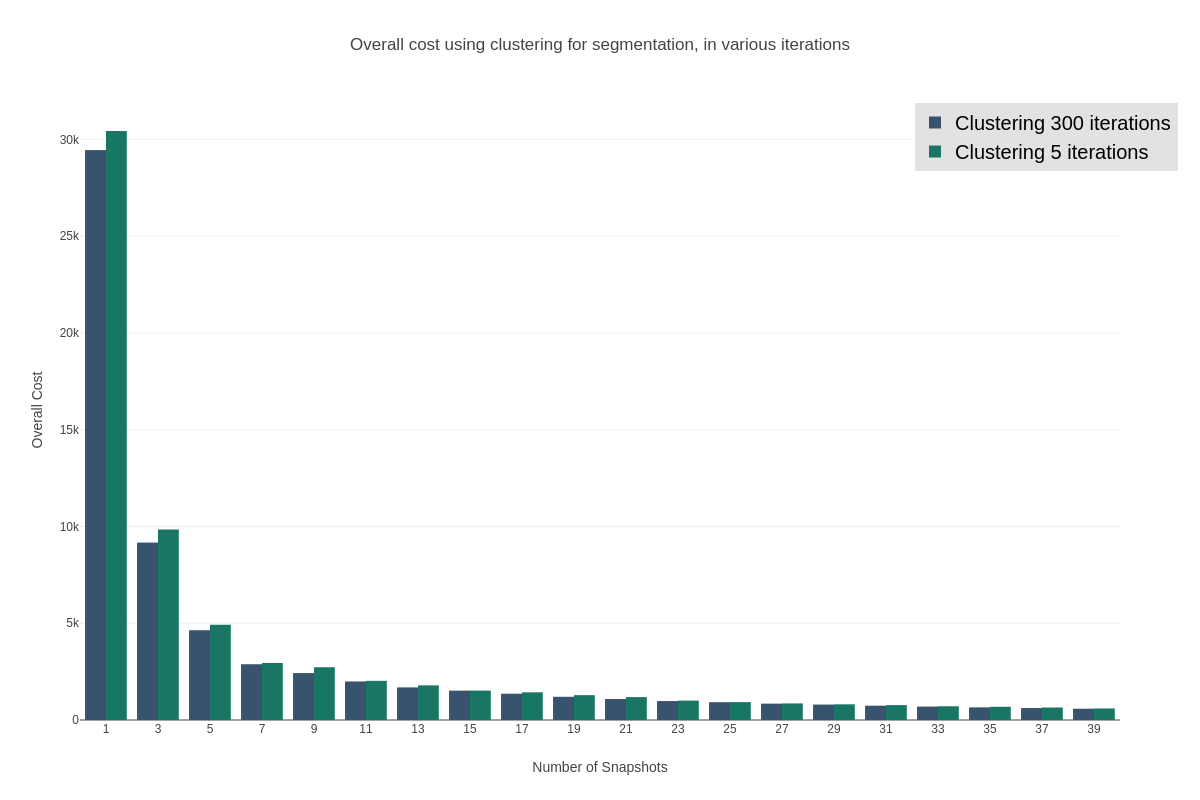
\includegraphics[width=\textwidth]{figs/compare_clustering_iterations.png}
				\caption{Comparing the overal cost of query answering in variable number of snapshots using K-Means clustering method with 30 and 300 iterations to find optimal timestamps for snapshots}
				\label{fig:compare_clusterings_iterations}
			\end{figure} 

			\begin {center}
			\begin{table}
				\centering
				\caption{A comparison between K-means clustering with 30 and 300 iterations}
				\label {table:compare_clustring_iterations}
				\begin{tabular}{p{2cm}p{3cm}p{3cm}p{3cm}}
					\hline
					Snapshots  & 300 iterations & 5 iterations \\ \hline
					1 & 29439.26 & 30439.26 \\  
					3 & 9159.13  & 9841.13\\
					5 & 4630.08  & 4921.08\\
					7 & 2867.74  & 2945.76\\
					9 & 2412.62  & 2732.38\\
					11 & 1980.95  & 2023.24\\
					13 & 1673.32  & 1789.50\\
					15 & 1509.57  & 1521.68\\
					17 & 1351.44  & 1430.66\\
					19 & 1194.61  & 1284.61\\
					21 & 1079.71  & 1182.71\\
					23 & 970.72  & 1002.57\\
					25 & 907.30  & 923.30\\
					27 & 836.97  & 856.83\\
					29 & 787.86  & 811.08\\
					31 & 731.61  & 769.83\\
					33 & 684.13  & 710.49\\
					35 & 640.58  & 683.60\\
					37 & 608.96  & 645.74\\
					39 & 575.97  & 595.89\\\hline
				\end{tabular}
			\end{table}
			\end{center}

		\section{Discussion}
			In this chapter the effectiveness of the proposed solutions to both lower the cost of queries on the temporal tables and add verifiability to the stored records in a database were put into experiment. We argued that the system could be developed by various tools but in order to generalize the application of our proposed methods for majority of relational databases, we chose the most favorable programming languages and tools by developers.
			The effectiveness of the snapshot materialization was the first set of experiments which was carried out. The experiments proved our claim that for a single snapshot placement for materialization, the median of the perviousely performed queries is the most optimal timestamp. The experiments also showed that for calculating the multiple optimal segmentation of queries on the timeline, the heuristic method beats the recursive and dynamic programming method in terms of computational time complexity. Our experiments showed that although the optimal solution is not guaranteed in the heuristic method, but the results obtained by using this method are satisfactory. For the sake of reducing the computational time even more, we lowered the iteration of the heuristic method and the results obtained were still satisfactory.

			Briefly speaking, the advantages and disadvantages of utilizing recursive algorithm, dynamic programming and heuristic method could be shown in Table \ref{table:segmentation_comparison}. 
			\begin{center}
				\begin{table}
					\centering
					\small
					\caption{Comparison between the methods to create optimal segmentations}
					\label{table:segmentation_comparison}
					\begin{tabular}{p{4cm}p{4cm}p{4cm}}
						\hline
						method & Pros  & Cons  \\ \hline
						Recursive algorithm & Exact optimal solution & Expensive for large number of queries and segmentations   \\ \hline
						Dynamic programming & Exact optimal solution & Expensive for large number of queries and segmentations\\ 
						  & Cheaper than dynamic programming &    \\ \hline
						K-Means clustering & Fast in computation & optimal solution not guaranteed \\ \hline
					\end{tabular}
				\end{table}
			\end{center}
			